\chapter{Обзор аналогов}
    Как уже было отмечено ранее, 3D-сканеры находят применение во множестве областей и решают самые разные задачи. Поэтому на данный момент уже есть готовые устройства, позволяющие производить сканирование, и реализовано несколько методов сканирования, каждый из которых требует разные компоненты и ресурсы. Рассмотрим существующие аналоги таких устройств и соответствующие им методы. Ограничим выбор 3D-сканерами распространяющиеся по open-source модели, поскольку в нашем проекте важна низкая стоимость модуля.
    
    Определим критерии для сравнения устройств:
    
    \underline{\textit{Точность}} --- насколько результаты измерения отклоняются от реальных. Один из наиболее важных параметров сканеров. В зависимости от метода колеблется от единиц миллиметров до микрометров.
    
    \underline{\textit{Скорость}} --- насколько быстро производятся вычисления. Многие задачи требуют расчётов в реальном времени и этот критерий является критическим. Как правило Высокая скорость обработки сказывается на точности алгоритма или ограничивает применимость системы (универсальность), поскольку использует специфичные упрощения и аппроксимации.
    
    \underline{\textit{Диапазон измерений}} --- диапазон расстояний (глубины) на которую рассчитано устройство для обеспечения заданной точности. Как правило определяется физическими ограничениями метода и конструкцией. Например размеры матрицы камеры и угол обзора задают верхний порог измерений, а для методов основанных на регистрации импульсов света существует нижний предел измерений обусловленный высокой скоростью света.
    
    \underline{\textit{Габариты}} --- в зависимости от используемой технологии получаются различные габариты и конфигурации. В настоящее время существуют ручные сканеры довольно малых размеров, но также есть и “настольные”, более габаритные устройства.

    \section{Мобильные приложения}
        \begin{figure}[!ht]
            \centering
            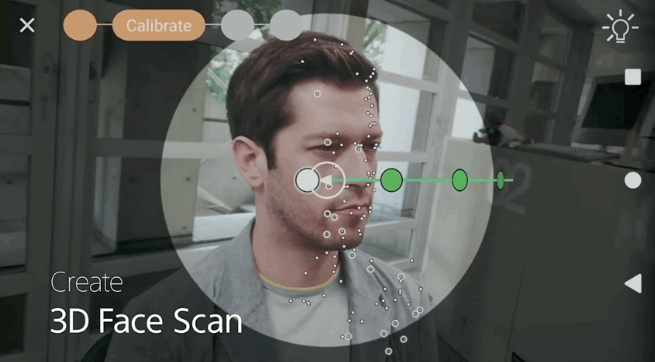
\includegraphics[width=0.5\linewidth]{sony3d}\label{pic:sony3d}
            \caption{Окно приложения Sony 3D creator}
        \end{figure}
        В настоящее время 3D-технологии довольно распространены, поэтому существуют приложения на смартфон (например, Sony 3D Creator), которые позволяют проводить сканирование любому человеку при наличии девайса поддерживающего необходимые технологии. Такие приложения как правило распространяются бесплатно, что делает её денежно самой выгодной (не считая стоимости смартфона).

        Эти приложения используют метод фотограмметрии для расчётов. Суть данного метода заключается в том, что, имея несколько изображений одного объекта с разных точек обзора, можно сопоставить особые точки (features) этих изображений после чего восстановить модель объекта по каждому пикселю снимков.

        Метод фотограмметрии, стереоскопия в частности, как правило имеет сравнительно низкую точность, но высокую скорость сканирования. Особенно низкая точность свойственна мобильным приложениям в виду ограниченных вычислительных ресурсов и качества используемых камер. Измерять таким методом можно объекты на расстоянии порядка метра от точки обзора. Габариты ограничены корпусом смартфона, однако этот же метод можно использовать с несколькими фиксированными камерами, то же касается стоимости.

        \begin{table}[H]
            \centering
            \caption{Характеристики приложения Sony 3D creator}\label{table:sony3d}
            \begin{tabular}{|l|l|}\hline
                Метод&Фотограмметрия\\ \hline
                Диапазон&$\approx 1$ м\\ \hline
                Скорость&По завершению съёмки\\\hline
                Точность&$\approx 1$ мм\\ \hline
                Габариты&Корпус смартфона\\ \hline
                Стоимость&Бесплатно (стоимость смартфона)\\ \hline
            \end{tabular}
        \end{table}

    \section{BQ Ciclop DIY 3D Scanner}
        \begin{figure}[!ht]
            \centering
            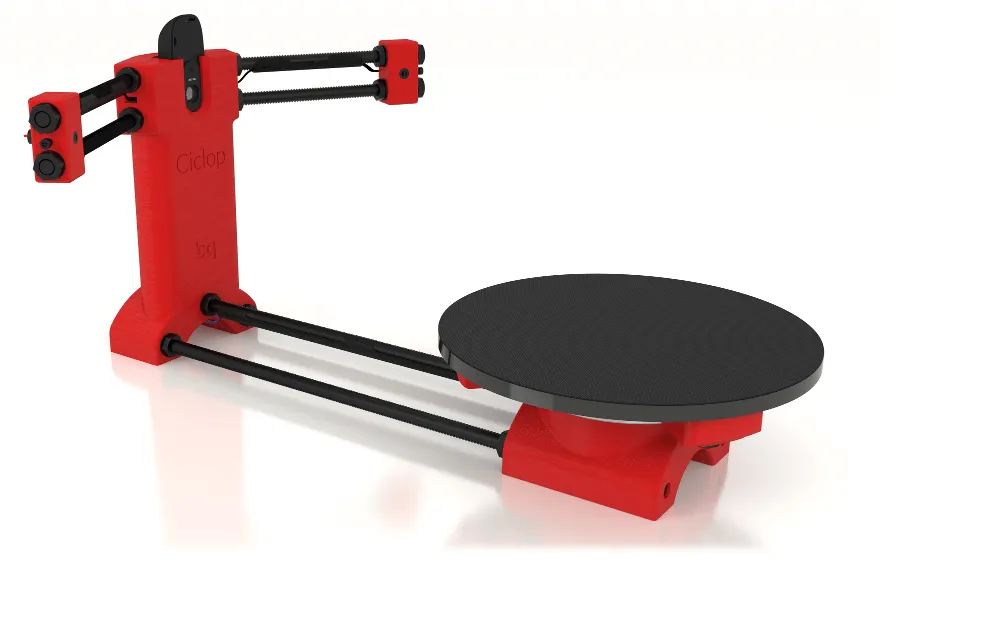
\includegraphics[width=0.5\linewidth]{ciclop}\label{pic:ciclop}
            \caption{Сканер BQ Ciclop}
        \end{figure}
        \lipsum[1-1]
        \begin{table}[H]
            \centering
            \caption{Характеристики сканера BQ Ciclop 3D Scanner}\label{table:ciclop}
            \begin{tabular}{|l|l|}\hline
            Метод&Лазерная триангуляция\\ \hline
            Диапазон&$\O250 \times 205$ мм\\ \hline
            Скорость&2-8 минут на оборот\\\hline
            Точность&$\approx 0.5$ мм\\ \hline
            Габариты&$ 500 \times 300 \times 230 $ мм\\ \hline
            Стоимость&6 000 р.\\ \hline
            \end{tabular}
        \end{table}

    \section{hesamh DIY 3D Scanner}
        \begin{figure}[!ht]
            \centering
            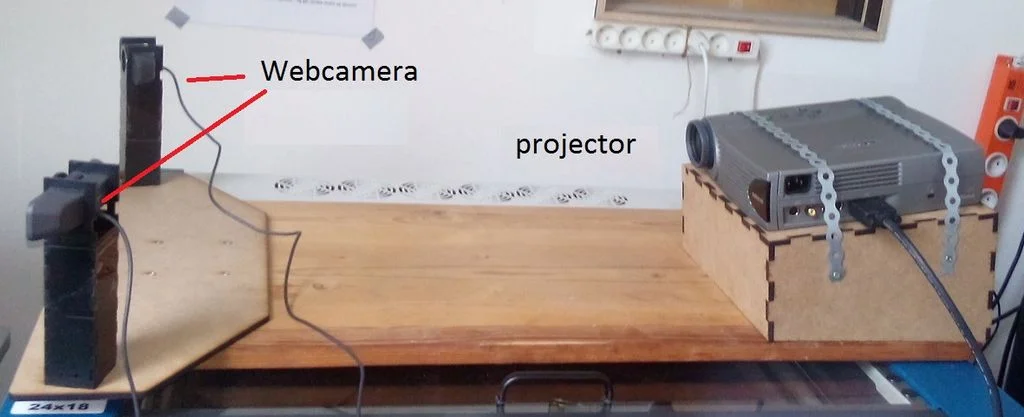
\includegraphics[width=0.5\linewidth]{hesamh}\label{pic:hesamh}
            \caption{Сканер hesamh}
        \end{figure}
    [Методы сканирования]
    [Сравнительная таблица? Какой-то итог]